\section{Terminologie des files d'attente}
La théorie des files d'attente étudie les systèmes et les processus d'attente en fonction de trois concepts clés:
\begin{itemize}
\item les \textbf{clients} (utilisateurs) sont les unités de travail désservies par le système -- un client peut être une personne réelle, ou il peut s'agir de tout ce que le système est censé traiter et compléter: une requête web, une requête de base de données, une pièce à usiner par une machine, etc;
\item les \textbf{serveurs} (ou guichets) sont les objets qui effectuent le traitement -- un serveur peut être le caissier de l'épicerie, un serveur web, un serveur de base de données, une fraiseuse, etc., et 
\item les \textbf{queues} (ou files d'attente) sont les endroits où les unités de travail attendent lorsque le serveur est occupé et ne peut pas commencer le travail dès leur arrivée -- une file d'attente peut être une ligne d'attente physique, elle peut résider en mémoire, etc. 
\end{itemize}
Afin de décrire les files d'attente, nous devons d'abord connaître et comprendre certaines distributions utiles, ainsi que les processus dît d'entrée-sortie.
\subsection{Distributions exponentielle et de Poisson}
Deux distributions jouent un rôle important dans la théorie des files d'attente. La distribution \textbf{de Poisson} compte le nombre d'événements discrets se produisant dans une période de temps fixe; elle est étroitement liée à la \textbf{distribution exponentielle} (et à la distribution Gamma), qui (entre autres applications) mesure le temps depuis l'arrivée d’un dernier événement. La distribution de Poisson est discrète; la variable aléatoire ne peut prendre que des valeurs entières non négatives. La distribution exponentielle peut prendre n'importe quelle valeur réelle non négative.
\par Considérons le problème de déterminer la probabilité que $n$ arrivées soient observées sur un intervalle de temps de longueur $t$, en supposant de plus que:
\begin{itemize}
\item la probabilité qu'une arrivée soit observée sur un petit intervalle de temps (disons de longueur $\nu$) est proportionnelle à la longueur de l'intervalle et que la constante de proportionnalité soit $\lambda$, de sorte que la probabilité devienne $\lambda\nu$;
\item la probabilité de deux ou plusieurs arrivées sur ce même petit intervalle est nulle, et 
\item le nombre d'arrivées dans un intervalle de temps donné est indépendant du nombre d’arrivées dans un intervalle qui ne le chevauche pas (par exemple, le nombre d'arrivées survenant entre 5 et 25 minutes depuis le départ ne fournit pas de renseignements sur le nombre d'arrivées survenant entre  30 et 50 depuis le départ).
\end{itemize}
\begin{figure}[!t]
\centering
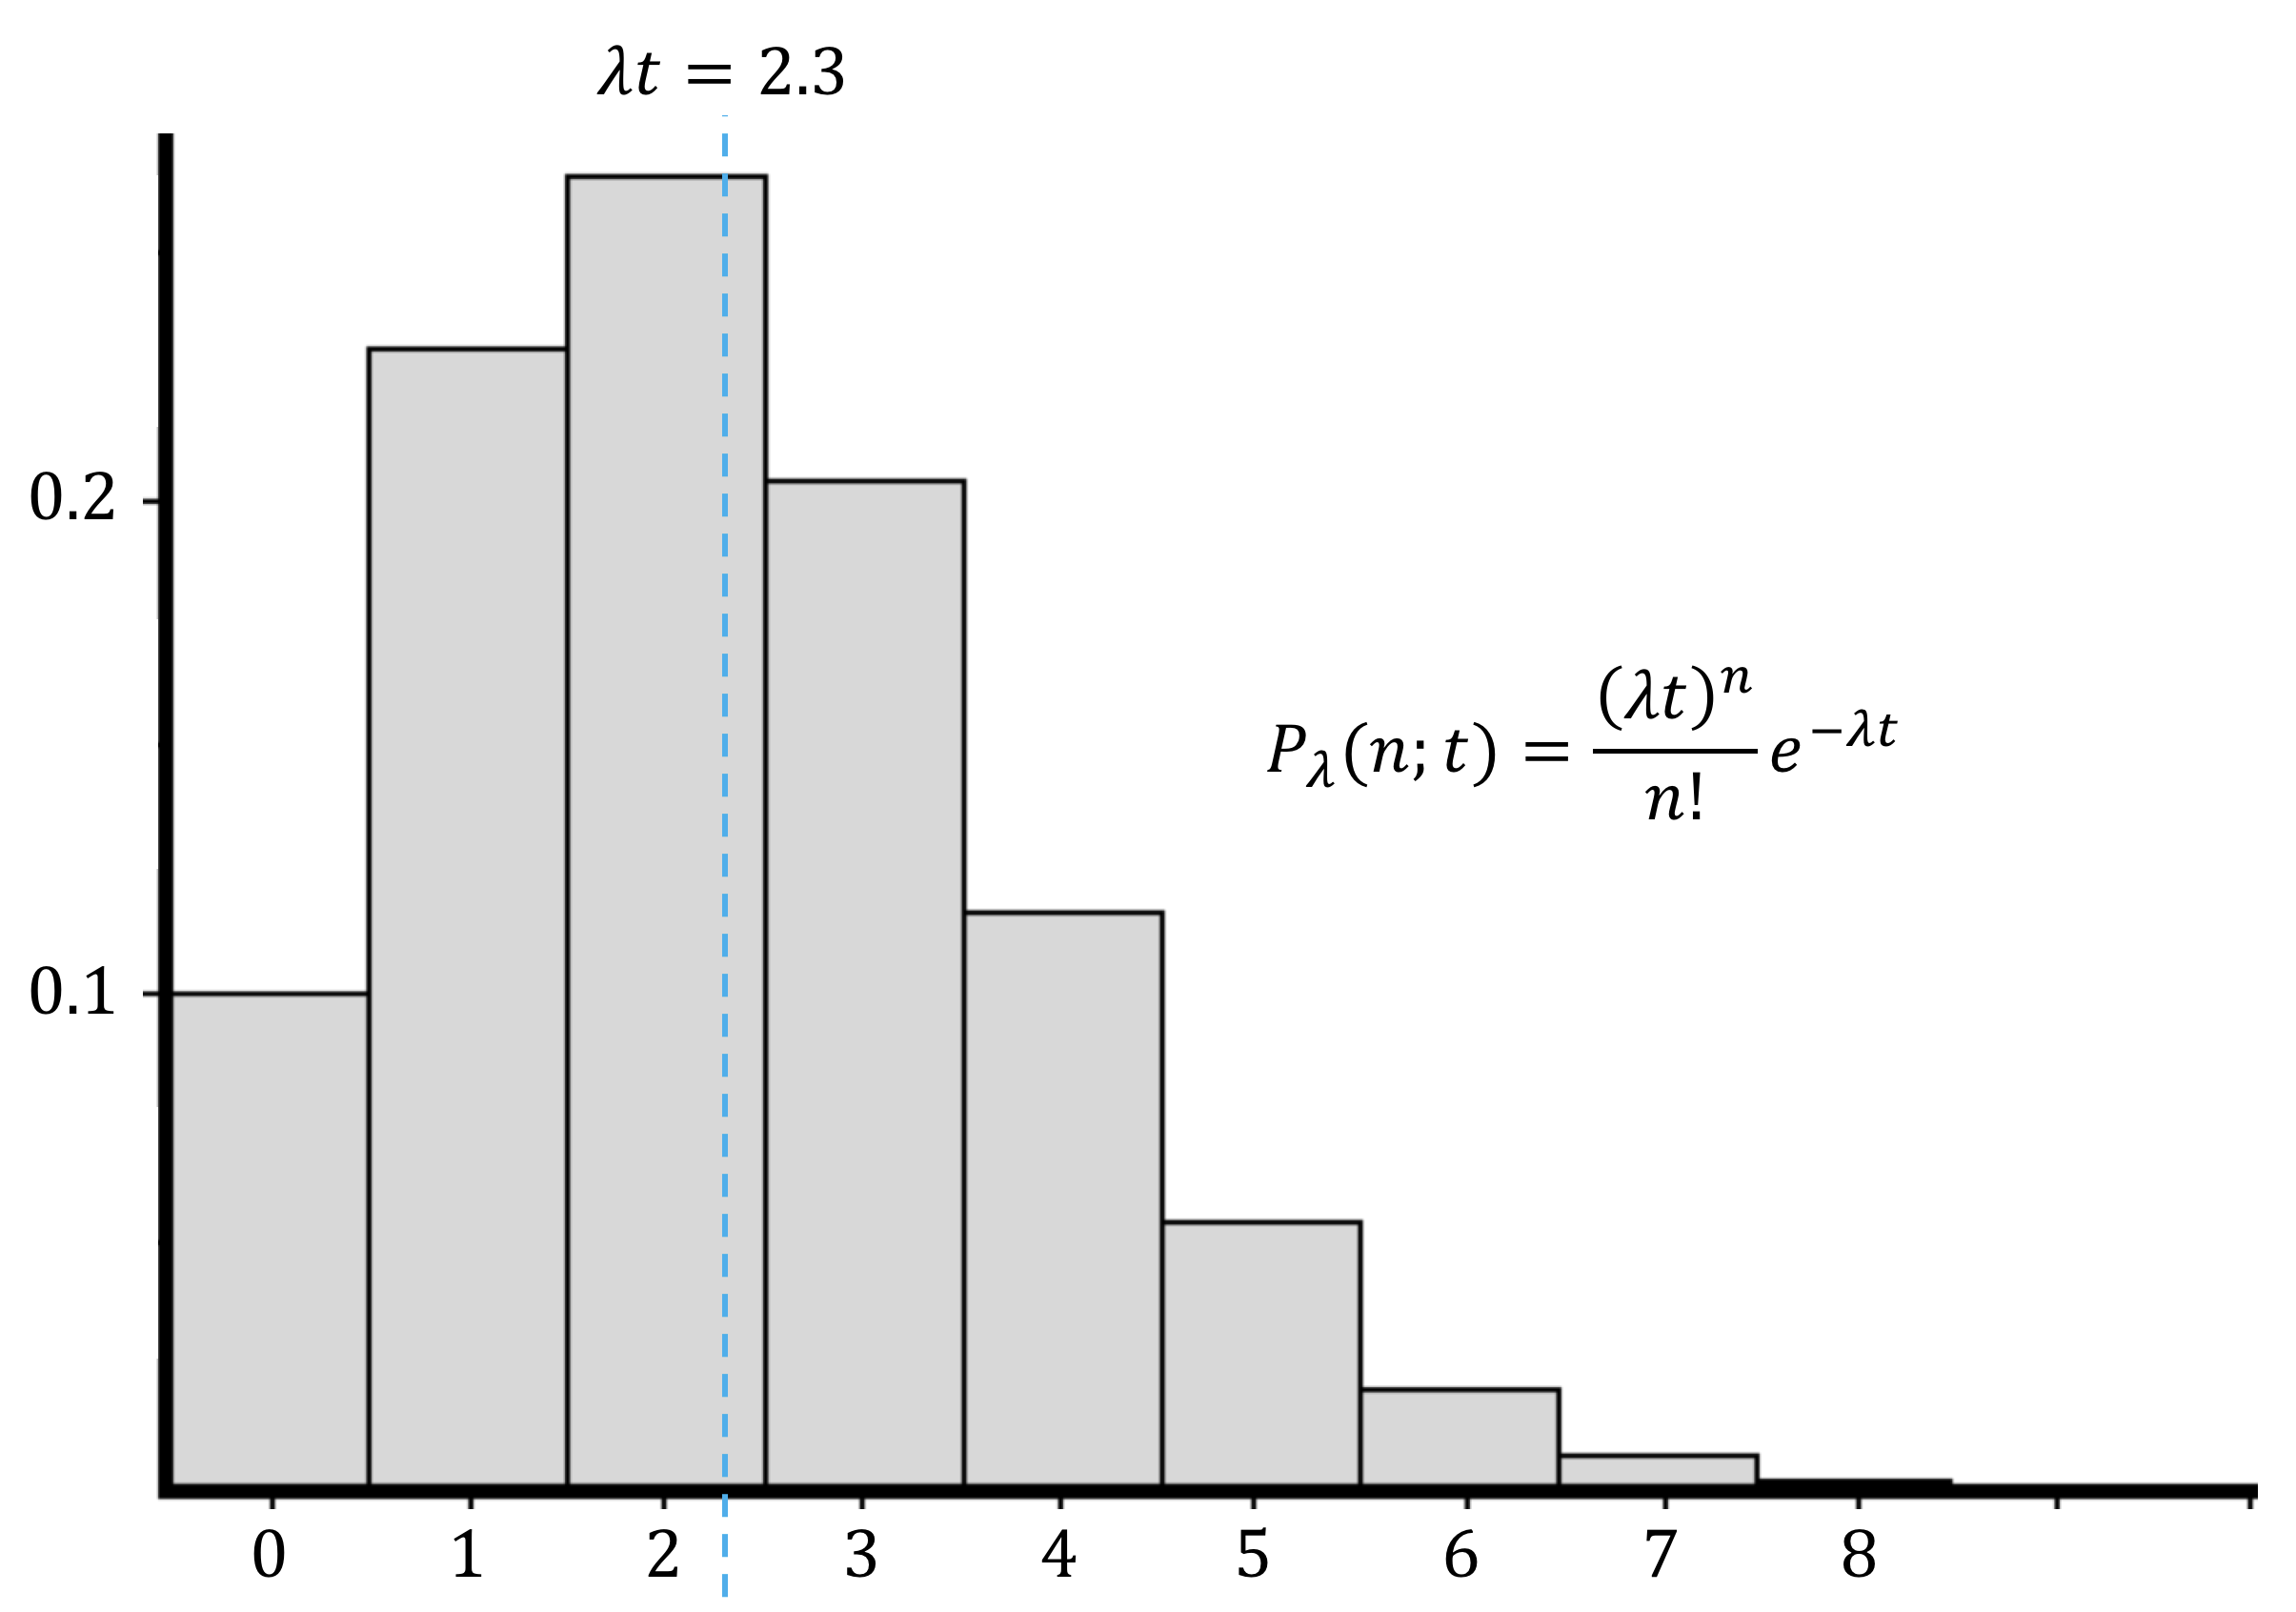
\includegraphics[height=0.25\textheight]{Images/poisson.png}
\centering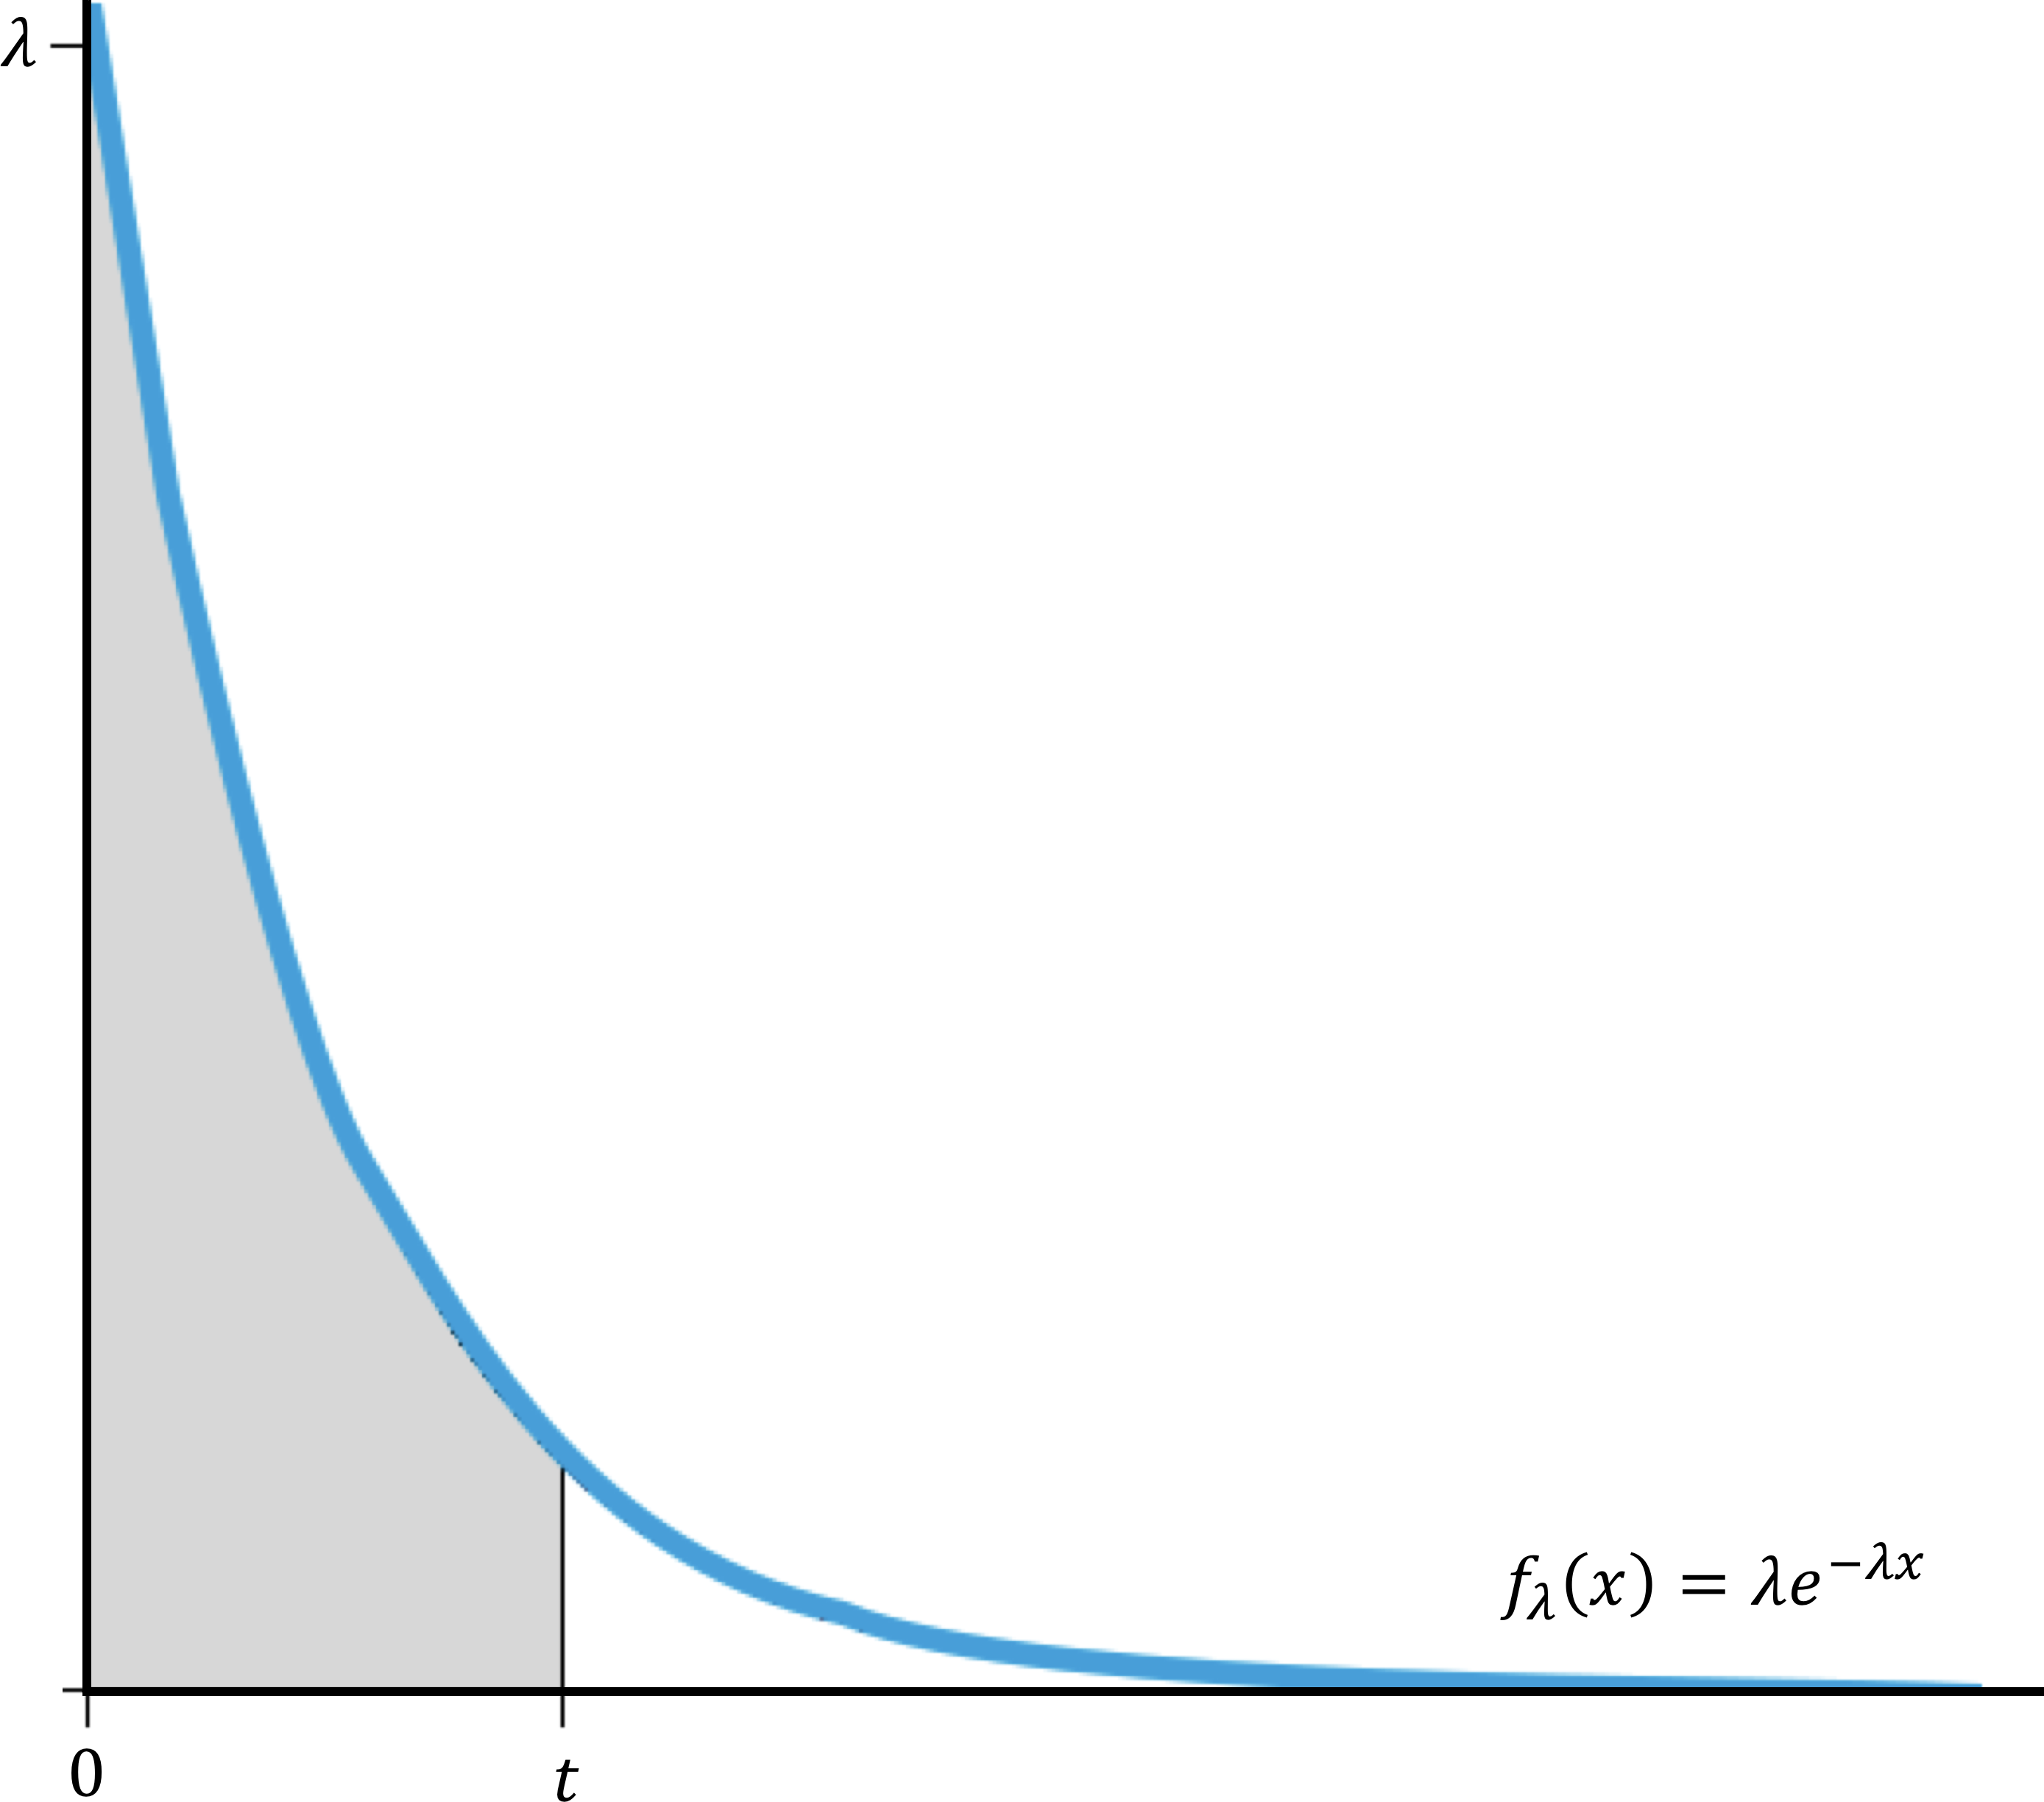
\includegraphics[height=0.25\textheight]{Images/exp.png}
\caption{\small Distribution de Poisson (avec $\lambda t=2.3$, en haut) et distribution exponentielle (avec  paramètre $\lambda$, en bas). La zone ombrée sur cette dernière représente la probabilité d’une attente de $t$ unités de temps si les arrivées sont Poisson de paramètre $\lambda$.}\label{fig:dist1}\hrule
\end{figure}
Soit $P(n;t)$ la probabilité d'observer $n$ arrivées dans un intervalle de temps de longueur $t$. La fonction de masse de la distribution du nombre d'arrivées est 
$$ P_{\lambda}(n; t) = \frac{(\lambda t)^n}{n!} e^{-\lambda t}, \ n=0,1,2,\cdots$$
pour un $\lambda>0$ spécifique au problème, c'est-à-dire que la distribution est Poisson (consulter la figure~\ref{fig:dist1}). Dans un système de file d'attente, ces arrivées sont dîtes \textbf{de Poisson}. \newl Le temps d’attente entre deux arrivées successives est l’\textbf{in\-ter\-val\-le d'ar\-ri\-vées}. Si le nombre d'ar\-ri\-vées dans un intervalle de temps donné suit une distribution de Poisson avec paramètre $\lambda t$, les intervalles d’arrivées suivent une distribution exponentielle, dont la fonction densité est donnée par 
$$ f_{\lambda}(t) = \lambda e^{-\lambda t}, \ \textrm{pour  }t>0,$$ et la probabilité $P(W\leq t)$ que le temps d'attente $W$ pour un utlisateur est inférieur à $t$ est 
$$P(W\leq t) = 1 - e^{-\lambda t}\quad \textrm{(consulter la Figure~\ref{fig:dist1})}.$$
De manière générale, si le taux d'arrivée est \textbf{stationnaire} et si il n’y a pas d'arrivées \textbf{en vrac} (c’est à dire qu’il n’y a pas d'arrivées simultanées), et si les arrivées passées n'affectent pas les arrivées futures, alors les intervalles d’arrivées suivent une distribution exponentielle avec paramètre~$\lambda$, et le nombre d'arrivées dans tout intervalle de longueur $t$ est Poisson avec paramètre $\lambda t$.
 \newl L'une des caractéristiques les plus intéressantes de la distribution exponentielle relative aux intervalles d'arrivées est qu'elle est \textbf{sans mémoire} -- si une variable aléatoire $X$ suit une distribution exponentielle, alors pour tout $t,h\geq 0$,
\begin{equation}
P(X \geq t + h|X \geq t) = P(X \geq h). 
\label{eq:1}
\end{equation}
C'est la seule fonction de densité qui satisfait à cette propriété~\cite{QS_R}. Cette propriété est importante car elle implique que la distribution des intervalles d'arrivées est indépendante du temps écoulé depuis la dernière arrivée -- imaginez si c'était le cas dans  les transports publics! \par Par exemple, si nous savons qu'au moins $t$ d'unités de temps se sont écoulées depuis la dernière arrivée, alors l’intervalle $h$ jusqu'à la prochaine arrivée est indépendante de $t$. Si $h=4$, disons, alors $(\ref{eq:1})$ donne 
$$ P(X>9|X>5)= P(X>7|X>3) = P(X>4).$$

\subsection{Distribution d'Erlang}
La distribution exponentielle n'est pas toujours un mo\-dè\-le approprié des intervalles d’arrivées; il n’est pas difficile d’imaginer une situation où le temps d’attente ne devrait pas être sans mémoire, par exemple. Une approche alternative utilise la distribution d'\textbf{Erlang} $\mathcal{E}(R,k)$, une variable aléatoire continue à deux paramètres $R>0$  $k\in \mathbb{Z}^+$,  dont la fonction de densité est  
$$ f_{R,k}(t) = \frac{R (Rt)^{k-1} e^{-Rt}}{(k-1)!},\ t\geq 0.$$
Lorsque $k=1$, la distribution d'Erlang se réduit à la distribution exponentielle $\text{Exp}(R)$. On peut aussi montrer que si $X\sim \mathcal{E}(k\lambda,k)$, alors $X\sim X_{1}+X_{2}+\cdots+X_{k},$ où chaque $X_{i}$ est une variable aléatoire exponentielle indépendente, de paramètre $k \lambda$. \newl En modélisant les intervalles d’arrivées selon une distribution d’Erlang $\mathcal{E}(k\lambda,k)$, nous disons de façon équivalente que les utilisateurs passent par $k$ \textbf{phases} (dont chacune est sans mémoire) avant d'être servi. Pour cette raison, le paramètre de forme est souvent appelé le nombre de phases de la distribution d'Erlang \cite{QS_N}.
\subsection{Arrivées et entrées}
Le processus de saisie est généralement appelé \textbf{processus d’arrivée}, les arrivées sont appelées \textbf{clients} (ou utilisateurs). Dans les modèles que nous considérerons, on supposent qu’il n’y a pas d'arrivées simultanées (ce qui peut être irréaliste lorsque l'on modélise les arrivées dans un restaurant, par exemple). Si des arrivées simultanées sont possibles (en théorie et/ou en pratique), nous disons des arrivées en vrac qu'elles sont \textbf{autorisées}. 
\par En général, nous supposons que le processus d'arrivée \textbf{n’est pas affecté par le nombre de clients} dans le système. Dans le contexte d'une banque, cela impliquerait que le processus régissant les arrivées reste inchangé, qu'il y ait 500 ou 5 personnes attendant qu’un guichet se libère. 
\newl Il existe deux situations courantes dans lesquelles le processus d'arrivée peut dépendre du nombre de clients présents. La première se produit lorsque les arrivées sont issues d'une petite population -- les modèles dits de \textbf{source limitée} -- si tous les membres de la population sont déjà dans le système, il ne peut y avoir une autre arrivée!\par Une autre situation de ce type se produit lorsque le taux auquel les clients arrivent dans l'établissement diminue lorsque celui-ci devient trop encombré. Par exemple, lorsque les clients constatent que le stationnement d'un restaurant est plein, ils peuvent très bien décider d'aller dans un autre restaurant ou de renoncer complètement à manger à l'extérieur. Si un client arrive mais ne parvient pas à entrer dans le système, nous disons que l'accès au système lui a été \textbf{bloqué}.
\subsection{Sorties et services}
Pour décrire le processus des sorties d’un système de file d'attente (souvent appelé \textbf{processus de service}), nous spécifions généralement une \textbf{distribution du temps de service}  qui régit le temps de service pour les  utilisateurs. \par Dans la plupart des cas, on suppose que cette distribution est indépendante du nombre de clients présents dans le système. Cela signifie, par exemple, que le serveur ne fonctionne pas plus vite lorsque lorsque le nombre de clients augmente.\newl On distingue deux types de serveurs: les serveurs  \textbf{en parallèle} et les serveurs \textbf{en série}. Les serveurs en parallèle fournissent tous le même type de service et les clients ne doivent passer que par l'un d'entre eux pour obternir un service complet. Les guichets d'une banque, par exemple, sont généralement disposés en parallèle; typiquement, les clients sont servis que par un seul guichet, et n'importe quel des  guichets peut offrir le service souhaité. \par Les serveurs sont en série si un client doit passer par plusieurs serveurs avant de terminer son service. Une chaîne de montage est un exemple d'un tel système de mise en file d'attente.
\newl 
On retrouve de tels processus dans diverses situations:
\begin{itemize}
\item \textbf{situation:} achater des billets pour les Blue Jays au centre Rogers\\ \textit{arrivées:} les partisans arrivent au guichet\\ \textit{sorties:} les guichetiers servent les acheteurs;
\item \textbf{situation:} pizzéria \\ \textit{arrivées:} les demandes de livraison de pizzas sont reçues \\\textit{output}: la pizzéria prépare et cuit des pizzas, et les envoie pour être livrées; 
\item \textbf{situation:} centre de services publics\\ \textit{input}: les citoyens/résidents entrent dans le centre de services \\ \textit{sorties:} la réceptionniste les affecte à une file d'attente spécifique en fonction de leurs besoins\\
\textcolor{white}{.}\qquad \textit{arrivées:} les citoyens/résidents se joignent à une \\ \textcolor{white}{.}\qquad file d'attente spécifique  \\ \textcolor{white}{.}\qquad \textit{sorties:} un fonctionnaire répond à leurs besoins;
\item \textbf{situation:} banque de sang à l'hôpital\\ \textit{arrivées:} les pintes de sang arrivent à l'hôpital\\ \textit{sorties:} les patients utilisent les pintes de sang selon leur type sanguin;
\item \textbf{situation:} garage\\ \textit{arrivées:} les voitures tombent en panne et sont envoyées au garage afin d'être réparées\\ \textit{sorties:} les voitures sont réparées par des mécaniciens et renvoyées sur les rues.
\end{itemize}
Les calculs pertinents sont assez faciles à exécuter, comme le montrent les exemples suivants.
\begin{Exemple} En moyenne, on s’attend à ce que 4.6 clients entrent dans un café durant chaque heure où il est ouvert. Si les arrivées respectent un processus de Poisson, la probabilité qu'au plus deux clients entrent pendant une période de 30 minutes (0.5 heures) est de \small \begin{align*}P_{4.6}&(n\leq 2;0.5)=P_{4.6}(0,0.5)+P_{4.6}(1,0.5)+P_{4.6}(2,0.5) \\ &=e^{-4.6\cdot 0.5}\left[\frac{(4.6\cdot 0.5)^0}{0!}+\frac{(4.6\cdot 0.5)^1}{1!}+\frac{(4.6\cdot 0.5)^2}{2!}\right] \\ &\approx 0.5960; \end{align*}\normalsize la distribution de Poisson correspondante peut \^etre consultée à la Figure~\ref{fig:dist1}.
\end{Exemple}
\begin{Exemple}
 Dans un fast-food, un caissier sert en moyenne 9 clients par heure. Si le temps de service suit une distribution exponentielle, $77.7\%$ et $1.1\%$ des clients seront servis en 10 minutes ou moins, et après 30 minutes, respectivement. En effet, \begin{align*}P(W\leq 10/60)&=1-e^{-9 \cdot 10/60} \approx 0.7769\\ P(W>30/60)&=e^{-9\cdot 30/60}\approx 0.0111.\end{align*}
\end{Exemple}

\subsection{Discipline de file d'attente}
Lorsque l’on cherche à décrire complètement un système de file d'attente, il faut aussi décrire sa \textbf{discipline} (ou de sa politique de service) et la manière dont les utilisateurs se  \textbf{joignent aux lignes}. La discipline de la file d'attente décrit la méthode utilisée pour déterminer l'ordre dans lequel les clients sont servis : 
\begin{itemize}
\item la politique de service la plus courante est celle dite du \textbf{premier arrivé, premier servi} (``first come, first served’’, FCFS), dans laquelle les clients sont servis dans l'ordre de leur arrivée, comme on s'attendrait à le voir dans un café d’Ottawa, par exemple;
\item sous la politique dite du \textbf{dernier arrivé, premier servi} (``last come, first served’’, LCFS), les derniers arrivés sont les premiers à entrer en service, comme c’est le cas dans un ascenseur bondé où tous les utilisateurs se rendent au même étage, par exemple;
\item parfois, l'ordre dans lequel les clients arrivent n'a aucun effet sur l'ordre dans lequel ils sont servis; ce serait le cas si le prochain client à entrer en service est choisi au hasard parmi les clients en attente de service, une situation appelée \textbf{service dans un ordre aléatoire} (``service in random order'', SIRO); 
\item enfin, la politique de \textbf{priorisation} place chaque arrivée dans une catégorie, chacune d'entre elles se voyant attribuer un niveau de priorité (un processus de \textbf{triage}); à l'intérieur de chaque niveau de priorité, les clients entrent dans la file d'attente sur une base FCFS; une telle politique de service est souvent utilisée dans les salles d'urgence afin de déterminer l'ordre dans lequel les clients sont traités, ou dans les services de reprographie et de partage de temps informatique, où la priorité est généralement accordée aux travaux dont les délais de traitement sont plus courts.
\end{itemize}

\subsection{Méthodes pour joindre la file d'attente}
Un autre facteur crucial dans le comportement du système de file d'attente est la \textbf{méthode} utilisée par les utilisateurs afin de déterminer à quelle ligne ils se joindront. Par exemple, dans certaines banques, les clients doivent se joindre à une seule ligne, mais dans d'autres, les clients peuvent choisir la ligne qu'ils souhaitent rejoindre. \par Lorsqu'il y a plusieurs lignes, les clients rejoignent souvent la ligne la plus courte. Malheureusement, dans de nombreuses situations (comme au supermarché, par exemple), il est difficile de définir quelle ligne est la plus courte, puisque le temps d’attente est aussi une fonction du nombres d’items dans les paniers des utilisateurs se trouvant déjà dans la ligne. S'il y a plusieurs lignes dans une installation de file d'attente, il est important de savoir si les clients sont autorisés à \textbf{changer} de ligne. Dans la plupart des systèmes de files d'attente à lignes multiples, le passage d’une ligne à l’autre  est autorisé, mais il n'est pas recommandé de le faire aux douanes, par exemple. 
